%
% fig-drehung.tex
%
% (c) 2025 Prof Dr Andreas Müller
%
\begin{figure}
\centering
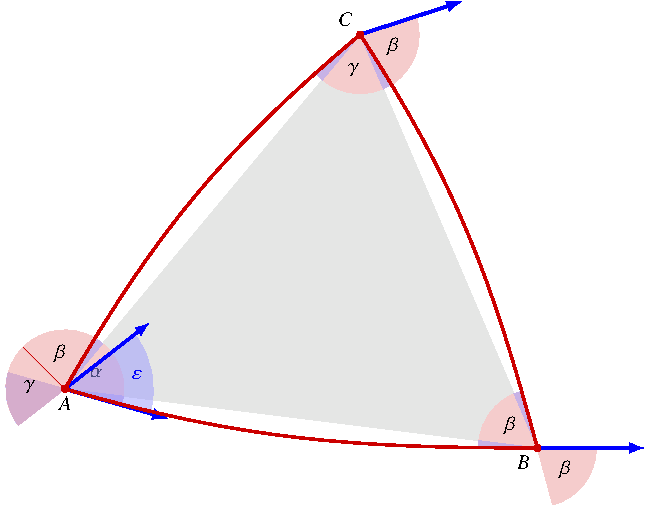
\includegraphics{chapters/110-kruemmung/images/drehung.pdf}
\caption{Die Drehung eines Vektors beim Paralleltransport eines
Tangentialvektors ausgehend vom Punkt $A$ entlang der Seiten eines
sphärischen Dreiecks entlang der Seiten des Dreiecks resultiert
in einer Drehung um den blauen Winkel.
Er ist gleich gross wie die Summe der in jeder Ecke eingezeichneten
kleinen blauen Winkel, die anzeigen, wieviel grösser die Winkel
des sphärischen Dreiecks sind als die des ebenen Dreiecks
$\triangle ABC$.
Ihre Summe heisst daher der sphärische Exzess
$\varepsilon = \alpha+\beta+\gamma-\pi$.
\label{buch:kruemmung:fig:drehung}}
\end{figure}
